%% XOP_Encoding_Paper.tex
%% V1.4b
%% 2015/08/26
%% by Eric Walkingshaw Jeffrey Young
%% See:
%% http://web.engr.oregonstate.edu/~walkiner/
%% for current contact information.
%%
%% This is a skeleton file demonstrating the use of IEEEtran.cls
%% (requires IEEEtran.cls version 1.8b or later) with an IEEE
%% conference paper.
%%

%%*************************************************************************
%% Legal Notice:
%% This code is offered as-is without any warranty either expressed or
%% implied; without even the implied warranty of MERCHANTABILITY or
%% FITNESS FOR A PARTICULAR PURPOSE! 
%% User assumes all risk.
%% In no event shall the IEEE or any contributor to this code be liable for
%% any damages or losses, including, but not limited to, incidental,
%% consequential, or any other damages, resulting from the use or misuse
%% of any information contained here.
%%
%% All comments are the opinions of their respective authors and are not
%% necessarily endorsed by the IEEE.
%%
%% This work is distributed under the LaTeX Project Public License (LPPL)
%% ( http://www.latex-project.org/ ) version 1.3, and may be freely used,
%% distributed and modified. A copy of the LPPL, version 1.3, is included
%% in the base LaTeX documentation of all distributions of LaTeX released
%% 2003/12/01 or later.
%% Retain all contribution notices and credits.
%% ** Modified files should be clearly indicated as such, including  **
%% ** renaming them and changing author support contact information. **
%%*************************************************************************


% *** Authors should verify (and, if needed, correct) their LaTeX system  ***
% *** with the testflow diagnostic prior to trusting their LaTeX platform ***
% *** with production work. The IEEE's font choices and paper sizes can   ***
% *** trigger bugs that do not appear when using other class files.       ***                          ***
% The testflow support page is at:
% http://www.michaelshell.org/tex/testflow/



\documentclass[conference]{IEEEtran}
% Some Computer Society conferences also require the compsoc mode option,
% but others use the standard conference format.
%
% If IEEEtran.cls has not been installed into the LaTeX system files,
% manually specify the path to it like:
% \documentclass[conference]{../sty/IEEEtran}

\usepackage{color}
\usepackage{enumerate}
\usepackage{lambda}

% Get todos to render properly
\usepackage[obeyFinal]{easy-todo}

% add package for ::= symbol, can't compile to pdf for some reason
% \usepackage{txfonts}

% add package for well rendered quotations
\usepackage{dirtytalk}

% Some very useful LaTeX packages include:
% (uncomment the ones you want to load)


% *** MISC UTILITY PACKAGES ***
%
%\usepackage{ifpdf}
% Heiko Oberdiek's ifpdf.sty is very useful if you need conditional
% compilation based on whether the output is pdf or dvi.
% usage:
% \ifpdf
%   % pdf code
% \else
%   % dvi code
% \fi
% The latest version of ifpdf.sty can be obtained from:
% http://www.ctan.org/pkg/ifpdf
% Also, note that IEEEtran.cls V1.7 and later provides a builtin
% \ifCLASSINFOpdf conditional that works the same way.
% When switching from latex to pdflatex and vice-versa, the compiler may
% have to be run twice to clear warning/error messages.






% *** CITATION PACKAGES ***
%
%\usepackage{cite}
% cite.sty was written by Donald Arseneau
% V1.6 and later of IEEEtran pre-defines the format of the cite.sty package
% \cite{} output to follow that of the IEEE. Loading the cite package will
% result in citation numbers being automatically sorted and properly
% "compressed/ranged". e.g., [1], [9], [2], [7], [5], [6] without using
% cite.sty will become [1], [2], [5]--[7], [9] using cite.sty. cite.sty's
% \cite will automatically add leading space, if needed. Use cite.sty's
% noadjust option (cite.sty V3.8 and later) if you want to turn this off
% such as if a citation ever needs to be enclosed in parenthesis.
% cite.sty is already installed on most LaTeX systems. Be sure and use
% version 5.0 (2009-03-20) and later if using hyperref.sty.
% The latest version can be obtained at:
% http://www.ctan.org/pkg/cite
% The documentation is contained in the cite.sty file itself.






% *** GRAPHICS RELATED PACKAGES ***
%
\ifCLASSINFOpdf
  \usepackage[pdftex]{graphicx}
  % declare the path(s) where your graphic files are
  \graphicspath{{../R/BellackTransTypology/Plots/}}
  % and their extensions so you won't have to specify these with
  % every instance of \includegraphics
  \DeclareGraphicsExtensions{.pdf,.jpeg,.png}
\else
  % or other class option (dvipsone, dvipdf, if not using dvips). graphicx
  % will default to the driver specified in the system graphics.cfg if no
  % driver is specified.
  % \usepackage[dvips]{graphicx}
  % declare the path(s) where your graphic files are
  % \graphicspath{{../eps/}}
  % and their extensions so you won't have to specify these with
  % every instance of \includegraphics
  % \DeclareGraphicsExtensions{.eps}
\fi
% graphicx was written by David Carlisle and Sebastian Rahtz. It is
% required if you want graphics, photos, etc. graphicx.sty is already
% installed on most LaTeX systems. The latest version and documentation
% can be obtained at: 
% http://www.ctan.org/pkg/graphicx
% Another good source of documentation is "Using Imported Graphics in
% LaTeX2e" by Keith Reckdahl which can be found at:
% http://www.ctan.org/pkg/epslatex
%
% latex, and pdflatex in dvi mode, support graphics in encapsulated
% postscript (.eps) format. pdflatex in pdf mode supports graphics
% in .pdf, .jpeg, .png and .mps (metapost) formats. Users should ensure
% that all non-photo figures use a vector format (.eps, .pdf, .mps) and
% not a bitmapped formats (.jpeg, .png). The IEEE frowns on bitmapped formats
% which can result in "jaggedy"/blurry rendering of lines and letters as
% well as large increases in file sizes.
%
% You can find documentation about the pdfTeX application at:
% http://www.tug.org/applications/pdftex





% *** MATH PACKAGES ***
%
%\usepackage{amsmath}
% A popular package from the American Mathematical Society that provides
% many useful and powerful commands for dealing with mathematics.
%
% Note that the amsmath package sets \interdisplaylinepenalty to 10000
% thus preventing page breaks from occurring within multiline equations. Use:
%\interdisplaylinepenalty=2500
% after loading amsmath to restore such page breaks as IEEEtran.cls normally
% does. amsmath.sty is already installed on most LaTeX systems. The latest
% version and documentation can be obtained at:
% http://www.ctan.org/pkg/amsmath





% *** SPECIALIZED LIST PACKAGES ***
%
%\usepackage{algorithmic}
% algorithmic.sty was written by Peter Williams and Rogerio Brito.
% This package provides an algorithmic environment fo describing algorithms.
% You can use the algorithmic environment in-text or within a figure
% environment to provide for a floating algorithm. Do NOT use the algorithm
% floating environment provided by algorithm.sty (by the same authors) or
% algorithm2e.sty (by Christophe Fiorio) as the IEEE does not use dedicated
% algorithm float types and packages that provide these will not provide
% correct IEEE style captions. The latest version and documentation of
% algorithmic.sty can be obtained at:
% http://www.ctan.org/pkg/algorithms
% Also of interest may be the (relatively newer and more customizable)
% algorithmicx.sty package by Szasz Janos:
% http://www.ctan.org/pkg/algorithmicx




% *** ALIGNMENT PACKAGES ***
%
%\usepackage{array}
% Frank Mittelbach's and David Carlisle's array.sty patches and improves
% the standard LaTeX2e array and tabular environments to provide better
% appearance and additional user controls. As the default LaTeX2e table
% generation code is lacking to the point of almost being broken with
% respect to the quality of the end results, all users are strongly
% advised to use an enhanced (at the very least that provided by array.sty)
% set of table tools. array.sty is already installed on most systems. The
% latest version and documentation can be obtained at:
% http://www.ctan.org/pkg/array


% IEEEtran contains the IEEEeqnarray family of commands that can be used to
% generate multiline equations as well as matrices, tables, etc., of high
% quality.




% *** SUBFIGURE PACKAGES ***
%\ifCLASSOPTIONcompsoc
%  \usepackage[caption=false,font=normalsize,labelfont=sf,textfont=sf]{subfig}
%\else
%  \usepackage[caption=false,font=footnotesize]{subfig}
%\fi
% subfig.sty, written by Steven Douglas Cochran, is the modern replacement
% for subfigure.sty, the latter of which is no longer maintained and is
% incompatible with some LaTeX packages including fixltx2e. However,
% subfig.sty requires and automatically loads Axel Sommerfeldt's caption.sty
% which will override IEEEtran.cls' handling of captions and this will result
% in non-IEEE style figure/table captions. To prevent this problem, be sure
% and invoke subfig.sty's "caption=false" package option (available since
% subfig.sty version 1.3, 2005/06/28) as this is will preserve IEEEtran.cls
% handling of captions.
% Note that the Computer Society format requires a larger sans serif font
% than the serif footnote size font used in traditional IEEE formatting
% and thus the need to invoke different subfig.sty package options depending
% on whether compsoc mode has been enabled.
%
% The latest version and documentation of subfig.sty can be obtained at:
% http://www.ctan.org/pkg/subfig




% *** FLOAT PACKAGES ***
%
%\usepackage{fixltx2e}
% fixltx2e, the successor to the earlier fix2col.sty, was written by
% Frank Mittelbach and David Carlisle. This package corrects a few problems
% in the LaTeX2e kernel, the most notable of which is that in current
% LaTeX2e releases, the ordering of single and double column floats is not
% guaranteed to be preserved. Thus, an unpatched LaTeX2e can allow a
% single column figure to be placed prior to an earlier double column
% figure.
% Be aware that LaTeX2e kernels dated 2015 and later have fixltx2e.sty's
% corrections already built into the system in which case a warning will
% be issued if an attempt is made to load fixltx2e.sty as it is no longer
% needed.
% The latest version and documentation can be found at:
% http://www.ctan.org/pkg/fixltx2e


%\usepackage{stfloats}
% stfloats.sty was written by Sigitas Tolusis. This package gives LaTeX2e
% the ability to do double column floats at the bottom of the page as well
% as the top. (e.g., "\begin{figure*}[!b]" is not normally possible in
% LaTeX2e). It also provides a command:
%\fnbelowfloat
% to enable the placement of footnotes below bottom floats (the standard
% LaTeX2e kernel puts them above bottom floats). This is an invasive package
% which rewrites many portions of the LaTeX2e float routines. It may not work
% with other packages that modify the LaTeX2e float routines. The latest
% version and documentation can be obtained at:
% http://www.ctan.org/pkg/stfloats
% Do not use the stfloats baselinefloat ability as the IEEE does not allow
% \baselineskip to stretch. Authors submitting work to the IEEE should note
% that the IEEE rarely uses double column equations and that authors should try
% to avoid such use. Do not be tempted to use the cuted.sty or midfloat.sty
% packages (also by Sigitas Tolusis) as the IEEE does not format its papers in
% such ways.
% Do not attempt to use stfloats with fixltx2e as they are incompatible.
% Instead, use Morten Hogholm'a dblfloatfix which combines the features
% of both fixltx2e and stfloats:
%
% \usepackage{dblfloatfix}
% The latest version can be found at:
% http://www.ctan.org/pkg/dblfloatfix




% *** PDF, URL AND HYPERLINK PACKAGES ***
%
%\usepackage{url}
% url.sty was written by Donald Arseneau. It provides better support for
% handling and breaking URLs. url.sty is already installed on most LaTeX
% systems. The latest version and documentation can be obtained at:
% http://www.ctan.org/pkg/url
% Basically, \url{my_url_here}.




% *** Do not adjust lengths that control margins, column widths, etc. ***
% *** Do not use packages that alter fonts (such as pslatex).         ***
% There should be no need to do such things with IEEEtran.cls V1.6 and later.
% (Unless specifically asked to do so by the journal or conference you plan
% to submit to, of course. )


% correct bad hyphenation here
\hyphenation{op-tical net-works semi-conduc-tor}


\begin{document}
%
% paper title
% Titles are generally capitalized except for words such as a, an, and, as,
% at, but, by, for, in, nor, of, on, or, the, to and up, which are usually
% not capitalized unless they are the first or last word of the title.
% Linebreaks \\ can be used within to get better formatting as desired.
% Do not put math or special symbols in the title.

\title{A Domain Analysis of Data Structure and Algorithm Explanations in the Wild}


% author names and affiliations
% use a multiple column layout for up to three different
% affiliations
\author{
\IEEEauthorblockN{Jeffrey Young}
\IEEEauthorblockA{School of EECS\\
Oregon State University\\
Corvallis, Oregon, USA}
\and
\IEEEauthorblockN{Eric Walkingshaw}
\IEEEauthorblockA{School of EECS\\
Oregon State University\\
Corvallis, Oregon, USA}
\and
\IEEEauthorblockN{Shujin Wu} 
% Can't get this to render right
% \IEEEoverridecommandlockouts \thanks{Now at Google} 
\IEEEauthorblockA{School of EECS\\
Oregon State University\\
Corvallis, Oregon, USA
}}

% TODO: add footnote indicating Shujin is now at Google


% conference papers do not typically use \thanks and this command
% is locked out in conference mode. If really needed, such as for
% the acknowledgment of grants, issue a \IEEEoverridecommandlockouts
% after \documentclass

% for over three affiliations, or if they all won't fit within the width
% of the page, use this alternative format:
% 
%\author{\IEEEauthorblockN{Michael Shell\IEEEauthorrefmark{1},
%Homer Simpson\IEEEauthorrefmark{2},
%James Kirk\IEEEauthorrefmark{3}, 
%Montgomery Scott\IEEEauthorrefmark{3} and
%Eldon Tyrell\IEEEauthorrefmark{4}}
%\IEEEauthorblockA{\IEEEauthorrefmark{1}School of Electrical and Computer Engineering\\
%Georgia Institute of Technology,
%Atlanta, Georgia 30332--0250\\ Email: see http://www.michaelshell.org/contact.html}
%\IEEEauthorblockA{\IEEEauthorrefmark{2}Twentieth Century Fox, Springfield, USA\\
%Email: homer@thesimpsons.com}
%\IEEEauthorblockA{\IEEEauthorrefmark{3}Starfleet Academy, San Francisco, California 96678-2391\\
%Telephone: (800) 555--1212, Fax: (888) 555--1212}
%\IEEEauthorblockA{\IEEEauthorrefmark{4}Tyrell Inc., 123 Replicant Street, Los Angeles, California 90210--4321}}




% use for special paper notices
%\IEEEspecialpapernotice{(Invited Paper)}




% make the title area
\maketitle

% As a general rule, do not put math, special symbols or citations
% in the abstract
\begin{abstract}
% A more problem-driven whack at it:
Explanations of data structures and algorithms are complex interactions of
several notations, including natural language, mathematics, pseudocode, and
diagrams. Currently, such explanations are created ad hoc using a variety of
tools, and the resulting artifacts are static reducing explanatory value. We
envision a domain-specific language for developing rich, interactive
explanations of data structures and algorithms. In this paper, we analyze this
domain to sketch requirements for our language. We build on an existing
pedagogic theory of explanation, which we adapt to a qualitative coding system
for explanation artifacts collected online. We show that explanations of
algorithms and data structures in the wild exhibit patterns predicted by the
pedagogic theory and derive insights for our language. This work is part of our
effort to develop the paradigm of explanation-oriented programming, which
shifts the focus of programming from computing results to producing rich
explanations of how those results were computed.
\end{abstract}

% no keywords




% For peer review papers, you can put extra information on the cover
% page as needed:
% \ifCLASSOPTIONpeerreview
% \begin{center} \bfseries EDICS Category: 3-BBND \end{center}
% \fi
%
% For peerreview papers, this IEEEtran command inserts a page break and
% creates the second title. It will be ignored for other modes.
\IEEEpeerreviewmaketitle



\section{Introduction}

Our high-level goal is to further develop the paradigm of explanation-oriented
programming (XOP). In XOP, the primary output of a program is not a set of
computed values, but an \emph{explanation of how} those values were computed.
However, programming languages for XOP should not merely produce explanations
as a byproduct, but should provide language features for manipulating
explanation objects directly, creating application-specific notations and
visualizations, and providing alternative explanations in response to user
queries. Additionally, the language should help guide the programmer toward the
creation of \emph{good} explanations.

As a step in this development, we aim to design and implement a domain-specific
language (DSL) in the XOP paradigm to support computer science education. The
intended users of the DSL are CS educators who want to create \emph{interactive
artifacts} to support the explanation of data structures and algorithms to CS
students. We envision these users as experts on the corresponding data
structures and algorithms, and also trained and skilled programmers. The
produced explanation artifacts might supplement a lecture or be posted to a web
page to supplement a textual explanation.

In this paper, we conduct a qualitative analysis of our domain, in order to
determine what kinds of explanation artifacts educators are already using, how
educators explain algorithms and data structures, and how these artifacts could
be improved on with more sophisticated tools (e.g.\ a DSL).

\subsection{Typologies of Explanation}

% This is bad, needs to be rewritten, ick I don't like it
Empirical branches of pedagogic theory have created, deployed, and analyzed
numerous ``coding systems'', known as \emph{typologies of
  explanation}~\cite{westbury1971research, nla.cat-vn407830,
  rosenshine1968objectively, hyman1968teaching, ennis1969logic,
  smith1967language, bellack1966language}. Typically, typologies are employed to
quantify methods of teaching, and thus can vary widely to suite the problem at
hand.

We translate one such Typology, created by Bellack et
al.\cite{bellack1966language} to explore patterns of explanation in static
explanatory objects, such as slideshow presentations and lecture notes. The
typology at hand was designed for exploring patterns of explanation that occur
in the discourse between a pupil and lecturer in a classroom setting. The
Typology's basic conceptual unit is called a \emph{pedagogical move}, which
represents a single step in the explanatory process. A series of cyclic
pedagogical moves constitute a \emph{teaching cycle}. Teaching cycles identify
\emph{how} a topic is being explained in a lecture. In general one can think of
them as representing the structure, cadence, and substance of a discourse
between a lecturer and a pupil. We employ the typology to observe and catalog
the teaching cycles in static explanatory documents created by universities and
then show how such a typology forms the basis for a DSL.

\subsection{Explanation Oriented Programming}
\todo{intro for XOP}

\subsection{Contributions}
This paper makes the following contributions:
%
\begin{enumerate}[C1.]

\item \label{contrib:codes}
%
We extend Bellack's system for analyzing \emph{explanation activities} in the
form of classroom discourse to support analyzing \emph{explanation artifacts}
in the form of lecture notes and slides.

\item \label{contrib:data}
%
We provide a coded qualitative data set of explanation artifacts, using the
system defined in \ref{contrib:codes}. The data set consists of \todo{XX}
explanations of Djikstra's shortest path algorithm and \todo{XX} explanations
of AVL Trees, collected from the Internet, see appendix A for a reference list
of sources.

\item \label{contrib:valid}
%
We provide evidence that our adaptation of Bellack's system to explanation
artifacts is sound since we can identify high-level patterns in artifacts
consistent with patterns in explanation activities coded in the original
system, such as \emph{teaching cycles}.

\item \label{contrib:valid}
%
We analyze the data set and observe that \todo{something about one-sided
discussion, hopefully some other insights that are relevant to designing a
DSL}.

\end{enumerate}

\section{Background}
\subsection{A Typology of Explanation}
In this section we present an overview of Bellack et al's typology. We describe
it's philosophical foundations, its basic unit of analysis - the
\emph{pedagogical move} - and elucidate the constituents that compose a given
move. It should be noted that this is not a exhaustive or comprehensive overview
of Bellack et al's typology, rather, this section is meant to familiarize the
reader with the basic structure of such a typology.

Bellack's system is founded upon, and formalizes rules to a \emph{language
  game}\cite{wittgenstein2010philosophical} that takes place between a pupil,
and a lecturer in a classroom setting. The consequent typology reflects this
foundation in terms of \emph{pedagogical moves}. A pedagogical move is the basic
unit of discourse in the pedagogic interlocution between pupil and lecturer.
Bellack et al. identify four types of pedagogical moves.
%
\begin{enumerate}[P1.]

  \item \label{contrib:struct}
    Structuring Move: a structuring move functions to \emph{set the context} for
    subsequent behavior. These are statements that a lecturer makes such as
    ``Let's move on to some examples'' or ``Lambda Calculus has simple
    operational semantics''.
  
  \item \label{contrib:solicit}
    Soliciting Move: A soliciting move is a verbal statement, made by the
    lecturer, which explicitly elicits a verbal response. These are statements
    such as ``Can anyone tell me the purpose of the dot operator?'' or ``Why is
    Depth-First Search better suited for certain game trees than Breadth-First Search?''

   \item \label{contrib:response}
     Response Move: A response move is reciprocal to a soliciting move, and only
     occur in relation to them. Response moves function to fulfill the
     expectation of soliciting moves. In short, these are the answer's to a
     lecturer's questions. Some examples are ``The dot operator represents
     function composition'' or ``Depth-First Search is memory efficient, while
     Breadth-First Search is not.''

   % what does contrib:XXX do?
   \item \label{contrib:react}
     Reacting Move: A reacting move are coincident with structuring, soliciting,
     and responding moves. Reacting moves are not directly elicited by any other
     move, but are still occasioned by them. These function to \emph{qualify}
     some former move through clarifying some point, expanding on some point, or
     even by synthesizing a new move altogether. Examples of these moves include
     % could probably use a more illustrative example, or we could use the free
     % trade example that Bellack employs.
     statements such as ``That's partly correct; Depth-First Search is more
     memory efficient but that is not the only reason..''

\end{enumerate}

The coding notation in Bellack et al's system consists of eight categories
separated by a ``/''. We have affixed each category with an index for
specificity and following Bellack's presentation . The eight categories are as
follows:
% any thoughts on how to get this in BNF, or even if we should?

\begin{enumerate}
  \item Speaker
  \item Type of Move
  \item Substantive Meaning
  \item Substantive-Logical Meanings
  \item Number of Lines in 3 or 4
  \item Instructional Meaning
  \item Instructional-Logical Meanings
  \item Number of Lines in 6 or 7
\end{enumerate}

% should this be ``the Semantics of each ...'''???
For each category a shorthand indicator is provided that details the
representation of that category in the terminology of the coding system.
For example a structuring move is represented as (STR) in the system's
notation. In this section we present the meanings of each category. We focus on
categories 1 - 5 for they constitute the bulk of the typology used in section
\todo{XX}. We refer the interested reader to Bellack et al's work for an
exhaustive presentation \cite{bellack1966language}.The meanings of each category are as follows:

\begin{enumerate}
  \item{Speaker}: Indicates the source of the utterance, is one of:
  \begin{enumerate}
    \item \emph{Teacher} (T)
    \item \emph{Pupil} (P)
    \item \emph{Audio-Visual Device} (A)
  \end{enumerate}
  \item{Type of Move}: Indicates which type move belongs to. See P1-P4 above.
  \item{Substantive Meaning}: reference to a subject matter topic
  \item{Substantive-Logical Meaning}: Indicate a reference to cognitive process involved
    in dealing with subject matter under study. This category has three major
    subcategories: \emph{Analytic Process}, \emph{Empirical Process},
    \emph{Evaluative Process}, each with their own subcategories:
  \begin{enumerate}
    \item{Analytic Process}: Use of language or established rules of logic.
    \begin{enumerate}
      \item \emph{Definining-Denotative} (DED): To define denotatively is to
        refer to the objects to which the term is applicable. One may think of
        this type of definition as citing which objects constitute the
        denotation of a term. For example, ``An AVL Tree is a type of Binary
        Search Tree''
      \item \emph{Defining-Connotative} (DEC): To define connotatively is to
        refer to characteristics or properties of some class or term. For example ``An
        AVL tree is a BST with specific height, insert, delete conditions''
      \item \emph{Defining-General} (DEF): To define generally is to provide the
        defining characteristics of a \emph{class} of objects \emph{and} to give
        an example of some item within that class. This category is also used
        when the type of definition is unclear.
      \item \emph{Interpreting} (INT): A verbal equivalent of a statement, slogan, aphorism, or proverb
      \end{enumerate}
    \item{Empirical Process}: Use of a sense experience as criterion of truth.
      \begin{enumerate}
      \item \emph{Fact-Stating} (FAC): A statement about what is, was, or will be without explanation or evaluation.
      \item \emph{Explaining} (XPL): a statement about relation between objects, events, principles, conditional inference, cause-effect, explicit comparison-contrast, statement of principles, theories or laws
      \end{enumerate}
    \item{Evaluative Process}: set of criteria or value system as basis for verification
      \begin{enumerate}
      \item \emph{Opining} (OPN): personal values for statement of policy, judgment or evaluation of event, idea, state of affairs, direct and indirect evaluation included
      \item \emph{Justifying} (JUS): reasons or argument for or against opinion or judgment
      \end{enumerate}
    \item \emph{Logical Process Not Clear} (NCL): represents a $\bot$ value for Substantive-Logical Meanings
    \end{enumerate}
  \item{Number of Lines in 3 and 4 above}
  \item{Instructional Meanings}: To reference factors related to classroom
    management. 
    % \begin{enumerate}
    %   \item \emph{Assignment} (ASG): language suggesting or requiring student activity; reports, tests, readings etc.
    %   \item \emph{Material} (MAT): Use of teaching aids and instructional devices
    %   \item \emph{Logical Process} (LOG): Function of language or rule of logic; reference to definitions or arguments, but not presentation of such
    %   \item \emph{Action-Cognitive} (ACC): Cognitive process, but not the language or logic of a specific utterance; thinking, knowing, understanding, or listening
    % \end{enumerate}
  \item{Instructional-Logic Meaning}: To reference the cognitive processes related
    to the distinctly didactic verbal moves in the instructional situation.
  % \begin{enumerate}
  %   \item{Analytic Process}: see (4) above
  %   \item{Empirical Process}: see (4) above
  %   \item{Evaluative Process}: includes the definitions in (4) above and:
  %   \begin{enumerate}
  %     \item{Rating}: reference to metacommunication; usually an evaluative reaction (REA)
  %     \begin{enumerate}
  %       \item \emph{Repeating} (RPT):  implicit positive rating when statement (STA) is repeated by another speaker; also for SOL to repeat a vocal action (ACV)
  %       \item \emph{Qualifying} (QAL): explicit reservation stated in rating; exception
  %       \item \emph{Not Admitting} (NAD): rating that rejects by stating the contrary; a direct refutation
  %     \end{enumerate}
%     \item Extra-logical Process (SOL): expecting physical action or when logical nature of verbal response cannot be determined. 
%     \begin{enumerate}
%       \item \emph{Performing} (PRF): asking, demanding; explicit directive or imperative
%       \item \emph{Directing} (DIR): SOL with or without stated alternatives; asking for directive, not permision for specific action
%       \item \emph{Extra-logical Process Not Clear} (NCL): represents a $\bot$ for extra-logical process
%     \end{enumerate}
%   \end{enumerate}
% \end{enumerate}
\item {Number of Lines in 6 and 7 above}
\end{enumerate}

An example coded move has this form:
\begin{verbatim}
       T/STR/MAN/XPL/4/PRC/FAC/2
\end{verbatim}

The interpretation is as follows:

%% This needs formatting help
\begin{flushleft}
\begin{verbatim}
       T / STR / MAN / XPL /  4  / PRC / FAC / 2
      (1)/ (2) / (3) / (4) / (5) / (6) / (7) /(8)
\end{verbatim}
\end{flushleft}

Which is taken to mean: A \emph{teacher} (1) makes a \emph{structuring} (2) move
in which they \emph{explain} (4) something about \emph{Tree Manipulation} (3) for
\emph{four} (5) lines of the transcript and also state \emph{facts} (7) about
classroom \emph{procedures} (6) for \emph{two} (8) lines of the transcript.

This encoding could be used for a statement by a teacher such as:

\say{Single
Rotation will not work for case two because after a single rotation is applied,
the tree will still not be balanced. Thus, double rotations are required to
handle case two and case three.}

\subsection{Teaching Cycles}
Teaching cycles are cyclic patterns or combinations of pedagogical moves. A
cycle begins with a structuring move (STR) or a soliciting move (SOL) and ends
with any move that precedes a new cycle. For example, the pattern ``STR SOL STR
STR'' has three teaching cycles in it: 1) STR SOL 2) STR and 3) STR. A teaching
cycle which has many of the same type of move referring back to a single STR
move is denoted as: ``STR REA REA \ldots''. Teaching cycles allow one to
describe pedagogical moves in relationship to each other. In Bellack's words:

\say{If a single pedagogical move may be compared to a move in chess or single
  play in football. Then teaching cycles may be seen as an interrelated series of move or plays}

The focus of teaching cycles is to be able to quantify linguistic events in the
classroom and combinations of pedagogical moves. \todo{decide if we need to
  espouse the 21 teaching cycles bellack identifies}

\section{Experimental Setup}
In this section we describe the nature of the data collected, the modifications
made to Bellack et al's typology and the criteria by which static explanatory
objects were collected.

\subsection{Modifications to the Typology}
The modifications made to Bellack et al's system are minor: we remove
the last 3 categories in Bellack's system (the categories that categorize
instructional material), we add one type of pedagogical move, two types of
substantive-logical meanings, and define substantive-meaning categories for each
algorithm:

\begin{enumerate}[M1.]
  \item{Categories} 
    \begin{enumerate}
      \item Location
      \item Type of Move
      \item Substantive Meaning
      \item Substantive-Logical Meanings
      \item Number of Slides of (c) and (d)
    \end{enumerate}
  \item{Additional Type of Move}
    \begin{enumerate}
      \item{Expositing Move:} An Expositing move is a type of pedagogical move
        that explicitly introduces or expands upon some information
    \end{enumerate}
  \item{Additional Substantive-Logical Meanings}
    \begin{enumerate}
      \item \emph{Visual Process} (VIS): an explicit visual representation is
        provided or serves as a discussion prompt.
      \item \emph{Defining-Operational} (DEO): to give a definition as a series
        of operations or steps affecting a state or machine. This is typically
        used to describe explicit presentations of programming code or pseudo-code.
    \end{enumerate}
  \item{Additional Substantive Meanings}
    \begin{enumerate}
      \item{AVL Trees}
        \begin{enumerate}
          % this language could be better
          \item \emph{Motivation} (MOT): refers to discussions of the motivations
            for what is being discussed
          \item \emph{Problems} (PRB): refers to explicit problems with whatever is
            being discussed.
          \item \emph{Tree} (TRE): refers to general discussion about an AVL
            Tree. When a move's substantive meaning is unclear or fits many
            meanings, this term is used.
          \item \emph{Traversal} (TRV): refers to discussion of how to traverse
            an AVL Tree
          \item \emph{Manipulation} (MAN): refers to discussion of operations to
            manipulate an AVL Tree. Any discussion of inserting, deleting or
            rotating is coded as MAN.
          \item \emph{Implementation} (IMP): refers to discussion of the actual
            implementation of an AVL tree. This may also refer to conditions or
            constraints which are necessary for the implementation of that which
            is being discussed.
        \end{enumerate}
      \item{Dijkstra's Algorithm}
        \begin{enumerate}
          % do you think we can get away with this?
          \item \emph{Motivation}: see section for AVL Trees
          \item \emph{Problems}: see section for AVL Trees
          \item \emph{Complexity} (COM): refers to the discussion of the computational
            complexity of that which is being discussed. 
          \item \emph{Application} (APP): refers to discussion of the application of
            that which is being discussed, whether it be concrete or abstract.
          \item \emph{Algorithm} (ALG): refers to general statements about the
            algorithm. When the substantive meaning is unclear or traverses many
            substantive meanings this term is used.
          \item \emph{Background} (BKG): refers to discussion of the history,
            background, people who created, were involved with, or are notable,
            for the thing being discussed.
        \end{enumerate}
      \item{MergeSort}
        \todo{Present the substantive categories for mergesort}
    \end{enumerate}
\end{enumerate}

The modifications made to Bellack et al's typology are largely orthogonal to the
original. While we did remove the last three categories, one could easily
imagine these being included and merely coded as $\bot$ or (NOC) in the original
typology. Any discussion of instructional material that was observed during
encoding was not considered and is not present in the data.

The largest changes are the addition of the expository step (EXP) and the visual
substantive-logical meaning (VIS). These were deemed necessary to employ the
typology to static objects. In a conversation, each interlocutor may solicit and
respond in turn, for static documents there simply is no way for a reacting or
responding move to take place. Thus, the language game between the reader and
the static document must be able to encompass the pure exposition of a subject
as a pedagogical move, hence the expository step was added.

Similar to the expository step, static documents such as power points or lecture
notes are able to communicate pedagogical information in a form not possible in
speech, viz. pictures, illustrations, animations or diagrams. In order to code
such unique pedagogical moves the visual step was added.

\subsection{Other Typologies of Explanation}
Pedagogic theory has many examples of typologies of explanation which are not
presented here. We adapt Bellack et al's because it is designed with the same
motivating research questions in mind as this work, namely quantifying
real-world examples of explanations. In this section, we will briefly review
alternative typologies and state our reasons for not adapting them. 

Brown and Armstrong\cite{brown1984explaining} developed a typology that sought
to qualify characteristics of \emph{good} explanations provided by teachers in a
classroom setting. Their typology was formed with two stated goals: 1) It should
be simple, elegant, and easy to pick up for student teachers and 2) It should be
powerful enough to characterize bad explanations from good ones, and relate to
previous pedagogic work. Their typology consists of ``keys'', which partition an
explanation, ``Links'' which form chains of keys that form the
explanation, and ``Rules'' which define any pertinent rules to for that which is
being explained. There are three categories of explanation in the typology: 1) The
Interpretative 2) The Descriptive and 3) The Reason Giving. While promising,
the presentation of this typology was deemed not formal enough to be actionable
for our purposes; for example, its presentation lacks definitions for significant terms
such as ``Links'' and ``Rules''. Furthermore, its desirable features are shared
with Bellack et al's typology viz. an explanation is a composition of some more
primitive concepts or categories.

%probably need an introductory sentence here
Roshenshine's\cite{rosenshine1968objectively} typology is generated through a
review of thirty lectures and the results of a user study. It's stated purpose
is to:

\say{objectively measured teaching behaviors that discriminate between more and
  less successful explanations of social studies material}. 

Rosenshine develops the grammar of terms based on a literature review of four
categories: 1) Linguistic Categories 2) Instructional Set 3) Presentational
categories and 4) Multivariate studies of teaching behaviors. Twenty one such
terms were identified and then tested in a user study for pedagogic impact. The
terms in the typology may include verbal and non-verbal behaviors in teachers.
While Rosenshines results were interesting the typology developed is
un-actionable for our purposes. The terms developed are either too broadly
defined, not translatable to a DSL, or by Rosenshines own research do not
correlate to a \emph{good} explanation. Furthermore, there is no set criteria
presented for encoding lectures with the typology. It is possible to adapt
Rosenshines work for our purposes but the resultant typology would differ so
radically from the original that it may no longer be relevant to Rosenshines own
work. Or to be succinct, Rosenshines typology is not easily extensible.

\section{Results}
In this section we present the method of data collection, the nature of the
data, and the criteria used to select explanatory objects. We then proceed to
present our findings. We make two major observations from the data: First,
we observe the presence of teaching cycles in static explanatory objects.
Secondly, we observe that the present typology's shortcomings are a limiting
factor to a more thorough investigation of explanatory objects.

% Should this be in experimental setup?
\subsection{The Data}
We restrict the scope of data collection to include only objects that provide an
explanation of common computer science algorithms from computer
science departments at accredited universities. Restricting the scope of objects
in this manner provides two benefits: 1) All explanatory objects have a stated,
intrinsic goal to communicate the mechanics, application, or implementation of
some common computer science algorithm. 2) There are bountiful and varied
examples of different approaches to explain \emph{the same} algorithm, and numerous
examples of \emph{like} approaches to explain different algorithms.

All data was coded by hand by individuals (coders) with access to a reference
document specifying the typology. Explanatory objects were indexed according to
the algorithm that was to be explained, and a simple counter. For example, the
first document regarding AVL Trees would be named ``AVL001'' while the sixth
would be ``AVL006'' and so on. All of the data analyzed in this paper was
collected by a single researcher. While we do not present an analysis of
agreement for this typology. In a predecessor typology we did observe a
significant agreement of \todo{show agreement percent} between two coders,
following the same procedures used to encode this data.

% Should I say more about the data pre-processing?
The data was pre-processed using R and Hadley Wickham's excellent ``dplyr'' library
\cite{Dplyr}, for the complete code see \todo{make github repo in lambda-land
  for paper resources}. In short, the pre-processing consists of creating an
``index'' variable that denotes the order a move was encoded in relation to each
document considered e.g. an index of 1 means that move happened immediately, and
sequentially, after the move indexed at 0. 

\subsection{Teaching Cycles}
To graphically observe, and represent, teaching cycles we form a dot plot for
each coded document, with lines connecting pedagogical moves that make up the
teaching cycle, as shown in Figure 1 below:

\todo{Make plot readable}
\begin{figure}[!h]
  \centering
  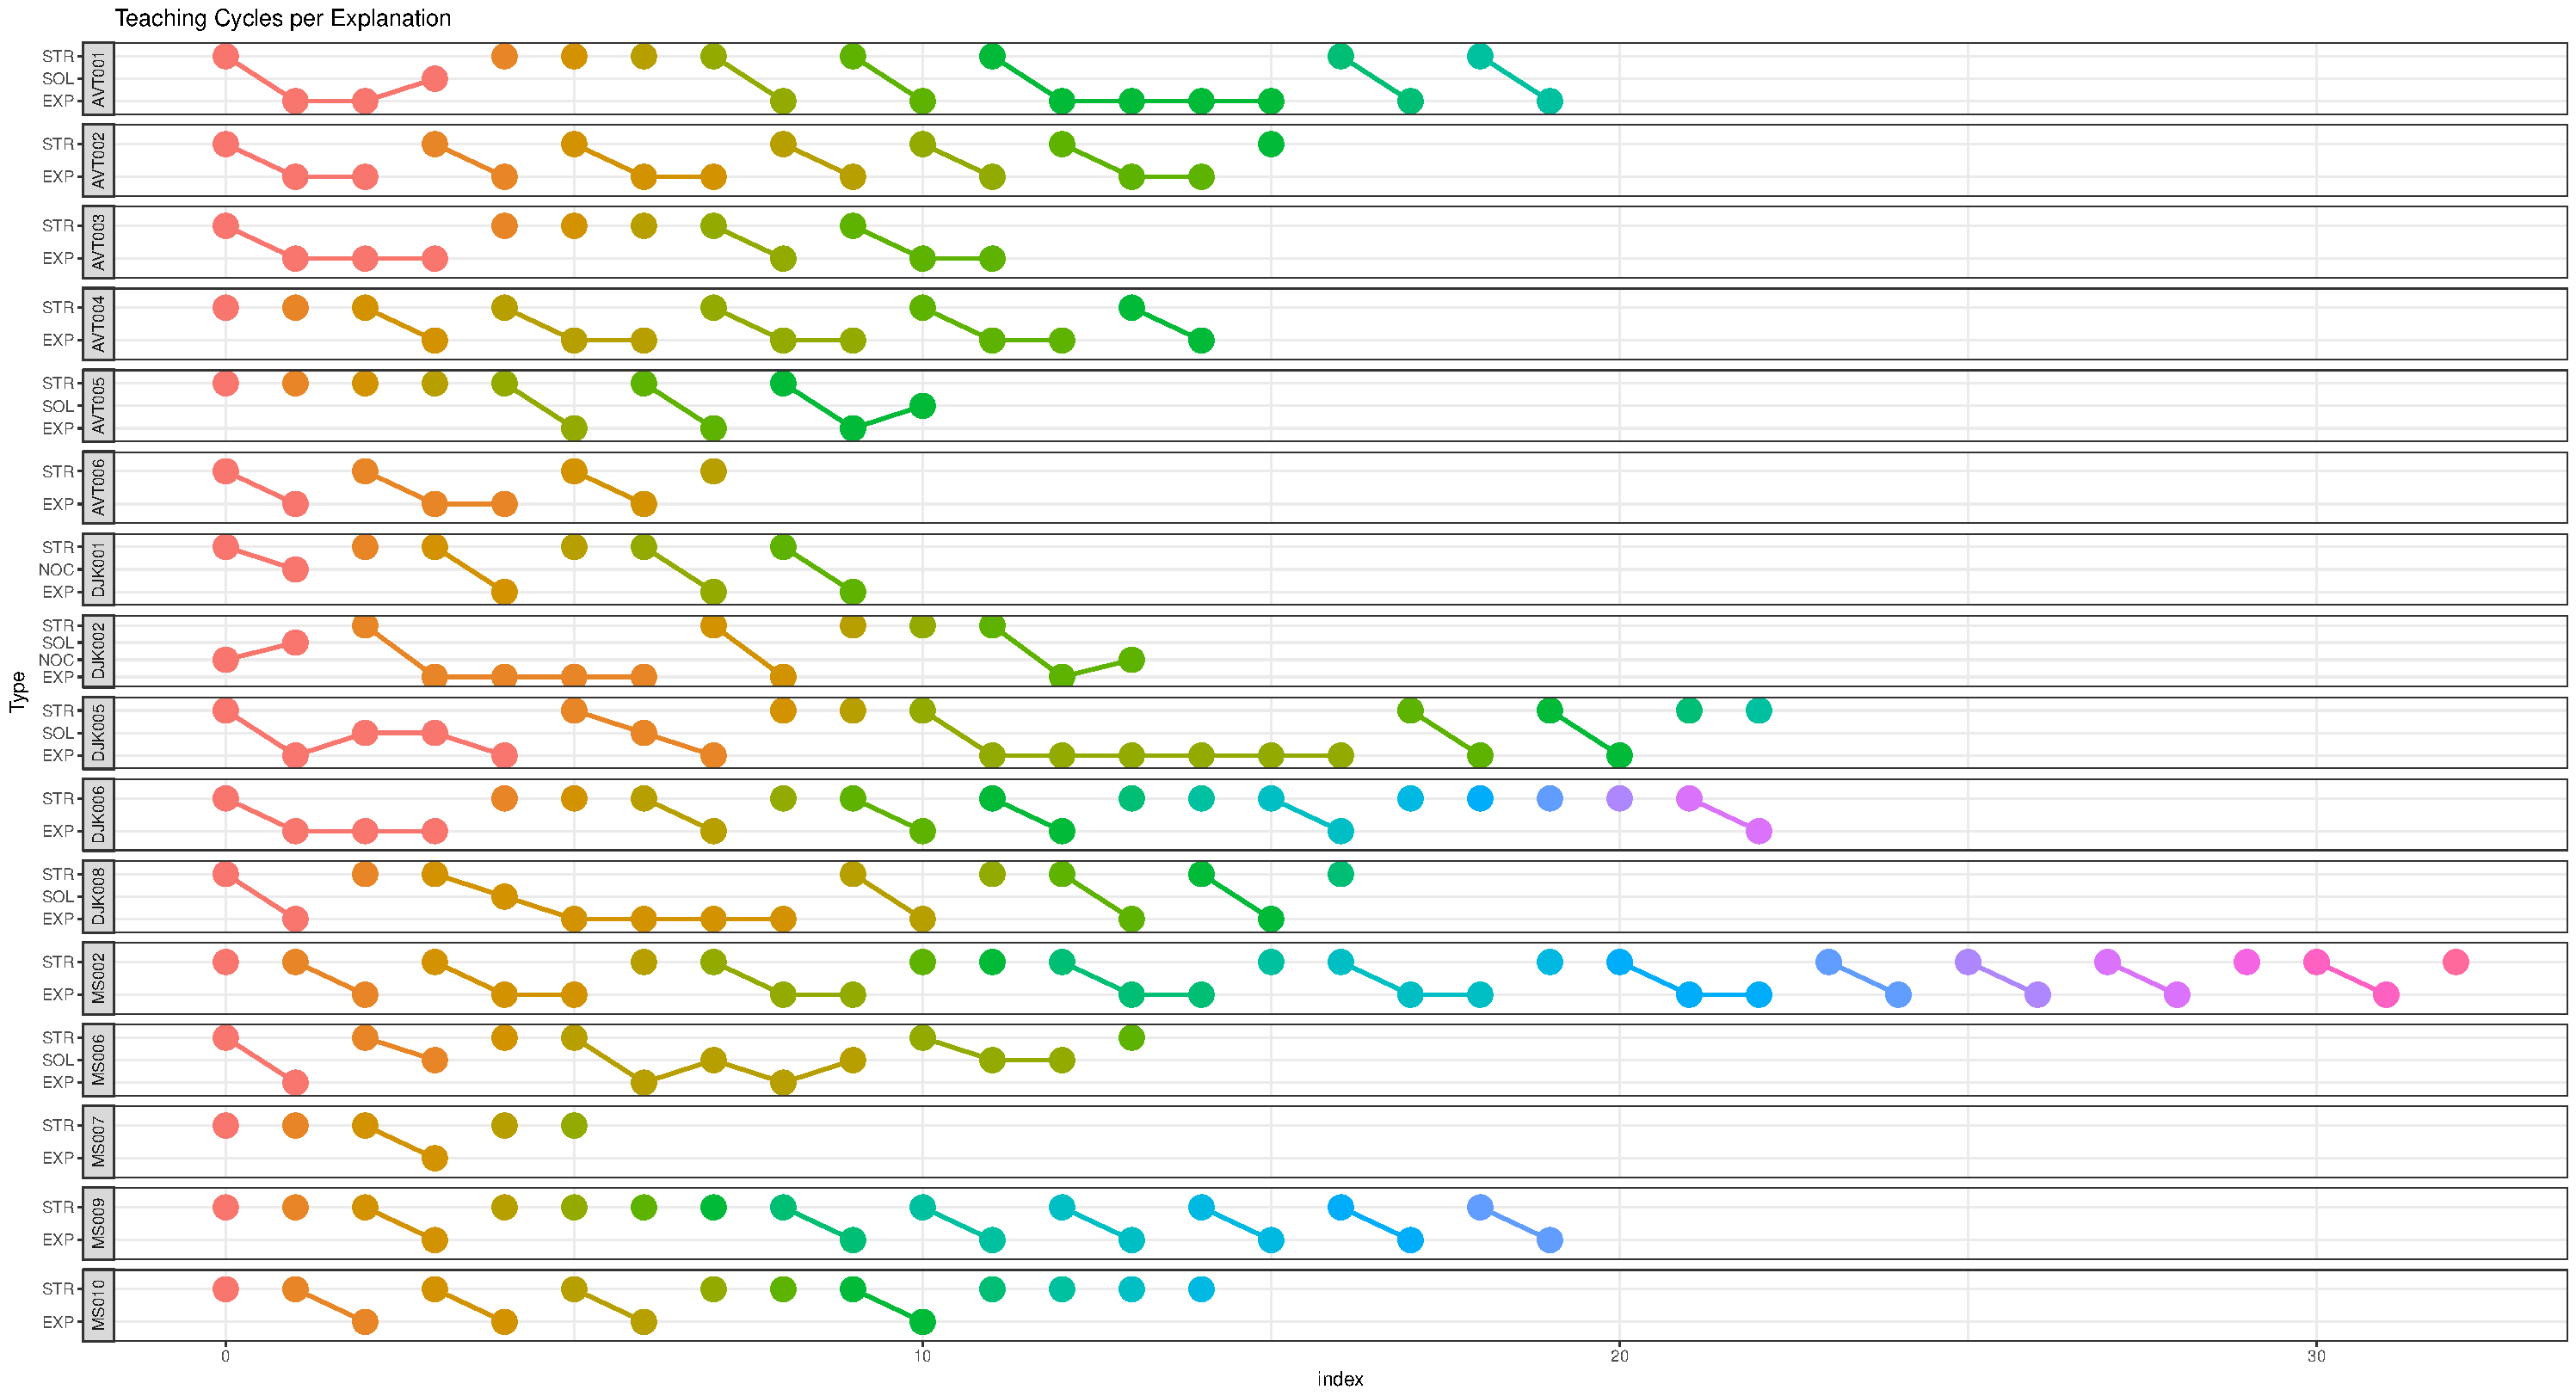
\includegraphics[width=2.5in]{teachCyclesPlt}
  \caption{Teaching cycles by Document}
  \label{fig:simple-empty}
\end{figure}

Each dot represents a single pedagogical move. The y-axis is faceted to display
the Type of Move for each coded document. For example ``AVL001'', the first
coded document for AVL Trees, has 3 types of pedagogical moves: STR, SOL, EXP.
One may also observe that this document has 4 different types of teaching cycles
viz. ``STR EXP SOL'', ``STR'', ``STR EXP'' and ``STR \emph{EXP}''.

Due to modifications to Bellack et al's typology we observe todo{XX} types
teaching cycles for static explanatory objects. These are shown in table 1 below:


% should we include NOC in the results?
  \begin{table}[h]
  \begin{center}
    \begin{tabular}{| l |}
      \hline
      Teaching Cycles \\ \hline
      STR \\ \hline
      STR NOC \\ \hline
      STR EXP \ldots \\ \hline
      STR EXP NOC \\ \hline
      STR EXP SOL \\ \hline
      STR SOL EXP \\ \hline
      STR SOL EXP \ldots \\ \hline
      STR EXP SOL \\ \hline
      STR EXP EXP SOL \\ \hline
      STR EXP SOL \\ \hline
      STR EXP SOL \ldots \\ \hline
      STR EXP NOC SOL \\ \hline
    \end{tabular}
    \caption{Observed Types of Teaching cycles in Static Documents,
      \emph{italics} denotes many}
  \end{center}
  \end{table}

\section{Discussion and Results}
In this section we summarize and interpret the results presented above. To
ensure transparency and openness, the reader may find all raw results published
online \todo{make repo holding raw results and R code}.

\subsection{Observed Teaching Cycles}
As shown in Figure 1, and listed in Table 1, we observe several types of
teaching cycles. Explanations in static documents adhere to a general pattern of
an introductory structuring (STR) move, followed by either a expositing (EXP) or
soliciting (SOL) move. Some cycles were \emph{atomic} in that they were isolated
to a single pedagogical move. These cycles are coded as a single STR move and
are synonymous with a single EXP move i.e. the document sets the context for an
explanation and then concludes the explanation within one \emph{unit} of the
document viz. a single slide for power point documents, or a single paragraph
for lecture notes. It is unsurprising that such atomic moves are observed with
more frequency in power point presentations than lecture notes. \todo{verify
  this claim after encoding lecture notes}

\subsection{Observed Typological Deficiencies}
Of particular note in our data is the \emph{absence} of any teaching cycle which
includes a responding (RES) or reacting (REA) move. Bellack et al's typology is
founded upon Wittgenstein's concept of a \emph{language game}. When applied to
discourse in the classroom such a foundation is easy to interpret. The lecturer
makes a move in the language game, and the pupil can then respond with a move of
their own. Bellack et al's typology captures the essence of this dynamic through
structuring, soliciting, responding and reacting moves. However, when applied to
a static document, the foundations of which the typology rest into conflict with
the nature of the document. Simply put, observing a responding or reacting move,
\emph{in} a static document would be nonsensical because the document has no way
to participate in the language game. Our analysis concludes this fact, as
expected, viz. that the modified typology, when applied to static documents,
constitute a category mistake regarding the foundations of the modified typology
of which it is based on. This fact may also be observed in the very
modifications made to Bellack et al's typology. The modifications to Bellack et
al's typology \emph{were required} in order to apply the typology to static
explanatory objects.

We believe that such deficiencies are promising ground for the creation of an
Explanation-Oriented DSL. One which would allow a static document \emph{to
  participate} in the language game. The modified typology presented in this
paper serves as a scaffold or paradigm from which to design such a DSL in a
semantics-first \cite{erwig2011semantics} manner.

\subsection{Applications to a DSL}

\section{Related Work}
% An example of a floating figure using the graphicx package.
% Note that \label must occur AFTER (or within) \caption.
% For figures, \caption should occur after the \includegraphics.
% Note that IEEEtran v1.7 and later has special internal code that
% is designed to preserve the operation of \label within \caption
% even when the captionsoff option is in effect. However, because
% of issues like this, it may be the safest practice to put all your
% \label just after \caption rather than within \caption{}.
%
% Reminder: the "draftcls" or "draftclsnofoot", not "draft", class
% option should be used if it is desired that the figures are to be
% displayed while in draft mode.
%
%\begin{figure}[!t]
%\centering
%\includegraphics[width=2.5in]{myfigure}
% where an .eps filename suffix will be assumed under latex, 
% and a .pdf suffix will be assumed for pdflatex; or what has been declared
% via \DeclareGraphicsExtensions.
%\caption{Simulation results for the network.}
%\label{fig_sim}
%\end{figure}

% Note that the IEEE typically puts floats only at the top, even when this
% results in a large percentage of a column being occupied by floats.


% An example of a double column floating figure using two subfigures.
% (The subfig.sty package must be loaded for this to work.)
% The subfigure \label commands are set within each subfloat command,
% and the \label for the overall figure must come after \caption.
% \hfil is used as a separator to get equal spacing.
% Watch out that the combined width of all the subfigures on a 
% line do not exceed the text width or a line break will occur.
%
%\begin{figure*}[!t]
%\centering
%\subfloat[Case I]{\includegraphics[width=2.5in]{box}%
%\label{fig_first_case}}
%\hfil
%\subfloat[Case II]{\includegraphics[width=2.5in]{box}%
%\label{fig_second_case}}
%\caption{Simulation results for the network.}
%\label{fig_sim}
%\end{figure*}
%
% Note that often IEEE papers with subfigures do not employ subfigure
% captions (using the optional argument to \subfloat[]), but instead will
% reference/describe all of them (a), (b), etc., within the main caption.
% Be aware that for subfig.sty to generate the (a), (b), etc., subfigure
% labels, the optional argument to \subfloat must be present. If a
% subcaption is not desired, just leave its contents blank,
% e.g., \subfloat[].


% An example of a floating table. Note that, for IEEE style tables, the
% \caption command should come BEFORE the table and, given that table
% captions serve much like titles, are usually capitalized except for words
% such as a, an, and, as, at, but, by, for, in, nor, of, on, or, the, to
% and up, which are usually not capitalized unless they are the first or
% last word of the caption. Table text will default to \footnotesize as
% the IEEE normally uses this smaller font for tables.
% The \label must come after \caption as always.
%
%\begin{table}[!t]
%% increase table row spacing, adjust to taste
%\renewcommand{\arraystretch}{1.3}
% if using array.sty, it might be a good idea to tweak the value of
% \extrarowheight as needed to properly center the text within the cells
%\caption{An Example of a Table}
%\label{table_example}
%\centering
%% Some packages, such as MDW tools, offer better commands for making tables
%% than the plain LaTeX2e tabular which is used here.
%\begin{tabular}{|c||c|}
%\hline
%One & Two\\
%\hline
%Three & Four\\
%\hline
%\end{tabular}
%\end{table}


% Note that the IEEE does not put floats in the very first column
% - or typically anywhere on the first page for that matter. Also,
% in-text middle ("here") positioning is typically not used, but it
% is allowed and encouraged for Computer Society conferences (but
% not Computer Society journals). Most IEEE journals/conferences use
% top floats exclusively. 
% Note that, LaTeX2e, unlike IEEE journals/conferences, places
% footnotes above bottom floats. This can be corrected via the
% \fnbelowfloat command of the stfloats package.




\section{Conclusion}
The conclusion goes here.




% conference papers do not normally have an appendix


% use section* for acknowledgment
\section*{Acknowledgment}


The authors would like to thank...





% trigger a \newpage just before the given reference
% number - used to balance the columns on the last page
% adjust value as needed - may need to be readjusted if
% the document is modified later
%\IEEEtriggeratref{8}
% The "triggered" command can be changed if desired:
%\IEEEtriggercmd{\enlargethispage{-5in}}

% references section

% can use a bibliography generated by BibTeX as a .bbl file
% BibTeX documentation can be easily obtained at:
% http://mirror.ctan.org/biblio/bibtex/contrib/doc/
% The IEEEtran BibTeX style support page is at:
% http://www.michaelshell.org/tex/ieeetran/bibtex/
%\bibliographystyle{IEEEtran}
% argument is your BibTeX string definitions and bibliography database(s)
%\bibliography{IEEEabrv,../bib/paper}
%
% <OR> manually copy in the resultant .bbl file
% set second argument of \begin to the number of references
% (used to reserve space for the reference number labels box)

\bibliography{XOPbib.bib}
\bibliographystyle{unsrt}

% that's all folks
\end{document}


